\documentclass{beamer}
\usepackage{amsmath}
\usepackage{verbatim}
\usepackage{graphicx}
\usepackage{xcolor}
\usepackage{listings}
\usepackage{tikz}
\usepackage{lipsum}
\usepackage{pgfplots}

\pgfplotsset{compat=1.18}


\usetheme{metropolis}           % Use metropolis theme
% Set the font to the default LaTeX font
\renewcommand{\familydefault}{\rmdefault}
\title{Designing Oscillator for an Antenna at \(\sim3.5[GHz]\)}

\date{}

\subtitle{2896}
\author{Mazz Shaikh(932056724), Nir Finch Cohen(230336612)}
\date{Edoh Shaulov}
\institute{Tel Aviv University}

% Define the logo image file
\newcommand{\mylogo}{
\includegraphics[height=1cm]{tau.jpg}} % Adjust the height as needed
\setbeamercovered{transparent}

% Change the color of the headings
\setbeamercolor{frametitle}{bg=gray!15, fg=black} % Adjust the color as needed

% Define the background template2
\setbeamertemplate{background}{
    \begin{tikzpicture}[remember picture,overlay]
        \fill[white] (current page.south west) rectangle (current page.north east); % White background
        \node[anchor=north east, inner sep=0pt] at (current page.north east) {\mylogo};
    \end{tikzpicture}
}
\begin{document}
\maketitle

% ----------------- section 1 --------------------

\section{Milestones completed so far}

\begin{frame}{List of Milestones completed}

  \begin{itemize}
    \item<1-> Selected the transistor we will use
    \item<2-> Simulated the oscillator we designed in PSpice
    \item<3-> Designed Matching network for the load(antenna)
    \item<4-> Optimised matching network for efficiency
  \end{itemize}
  
  

\end{frame}

% ----------------- section 1 --------------------




\section{Choosing the BJT}
\begin{frame}{Reqired characteristics}
  \begin{itemize}
    \item <1-> The transistor needs high-frequency performance, including \(f_{\text{max}}\) and \(f_t\), well above \(3.5[GHz]\).
    \item <2-> Low parasitic capacitance at collector, base, and emitter terminals is crucial.
    \item <3-> Low noise figure is essential.
    \item <4-> High gain, especially at the operating frequency, is necessary for stable oscillation.
    \item <5-> Ensure appropriate biasing for Colpitts oscillator operation, including DC voltages and currents.
  \end{itemize}
\end{frame}

\begin{frame}{Transistor Details}
\begin{center}
  \textbf{BFP520} from Infenion\footnote{\url{https://www.infineon.com/dgdl/Infineon-BFP520-DS-v02_00-EN.pdf?fileId=5546d462689a790c01690f035fe2391a}}
\end{center}
\begin{itemize}
  \item <2-> Surface mount low voltage silicon NPN RF bipolar transistor
  \item <3-> Transition frequency \(f_T\) of \(45[GHz]\)
  \item <4-> High Gain, with \(|S_{12}|, G_{ma}, G_{ms} > 16[dB]\) at \(3.5[GHz]\) under \(V_{ce} = 2[V]\)
  \item <5-> Low Noise Figure, \(NF < 1.2[dB]\) at \(3.5[GHz], 2[V], 2[mA]\)
\end{itemize}
\end{frame}

% ----------------- section 2 --------------------


\section{Oscillator Circuit}

\begin{frame}{Collpit's Oscillator}
\small
\begin{columns}
  \column{0.5\textwidth}
  \begin{itemize}
    \item <1-> The circuit was tested with some high impedance load attached
    \item <2-> Values of \(L_p\), \(C_1\) and \(C_2\) were computed using the operating frequency formula \[f_c\approx\frac{1}{2\pi\sqrt{L_p\frac{C_1C_2}{C_1+C_2}}}\] \footnote{In-depth analysis in Appendix}
    \item <3-> \(C_1=C_2\) was chosen since it gave the highest oscillation frequency
  \end{itemize}
  \column{0.5\textwidth}
  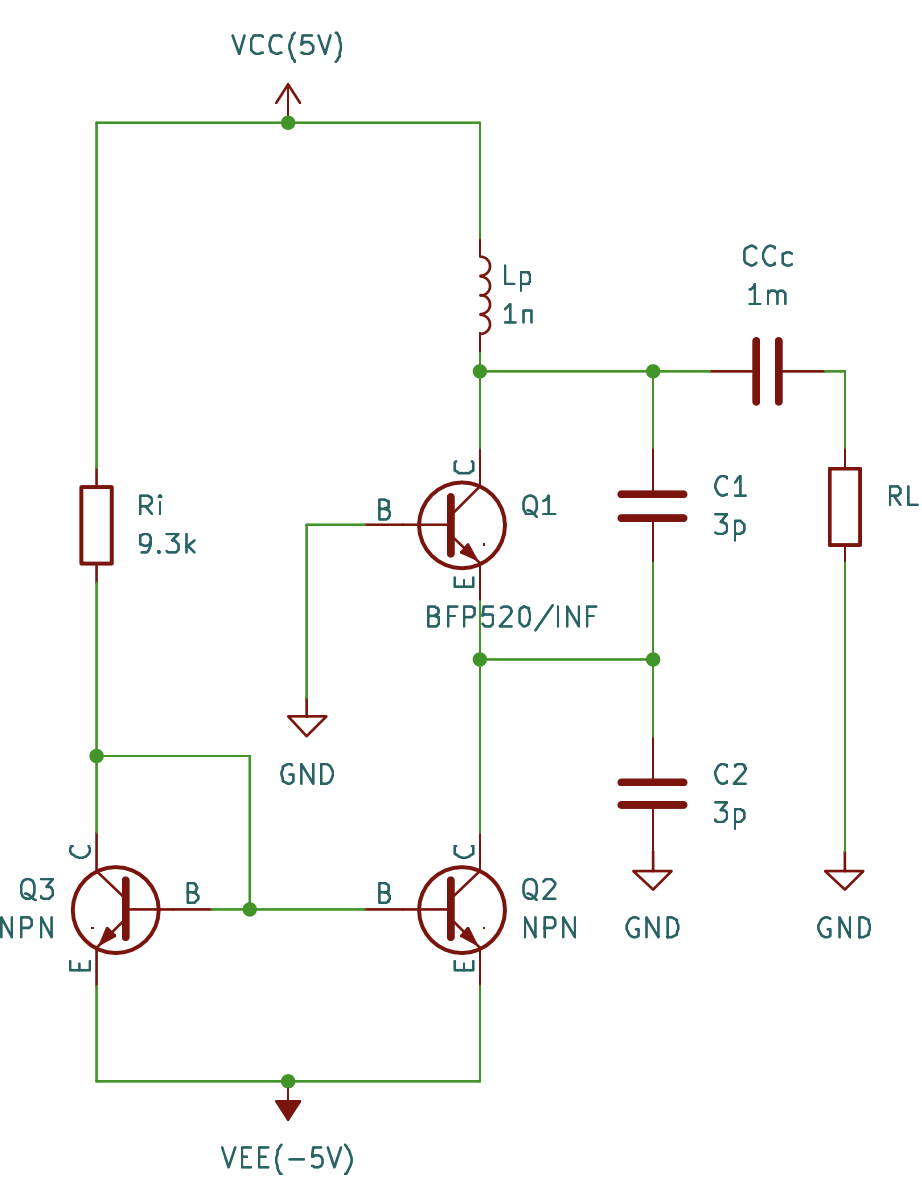
\includegraphics[width=0.95\linewidth]{images/collpits.png}
\end{columns}

\end{frame}

\begin{frame}{Ouput Waveform}


\end{frame}


% ----------------- section 3 --------------------

\section{Choosing a Matching Network}


\begin{frame}{Matching Network}

T-matching is better for matching a load to a source impedance when there's a large disparity because it provides efficient power transfer, minimizes losses, and offers impedance transformation with stability.\footnote{Design method in Appendix}
\begin{columns}
  \column{0.4\textwidth}

  \begin{itemize}
    \item \(L_{src} = 2.03361[nH]\)
    \item \(C_{src} = 2.02955[fF]\)
    \item \(L_{ld} = 10.4421[nH]\)
    \item \(C_{ld} = 0.208424[pF]\)
  \end{itemize}
  \column{0.6\textwidth}
  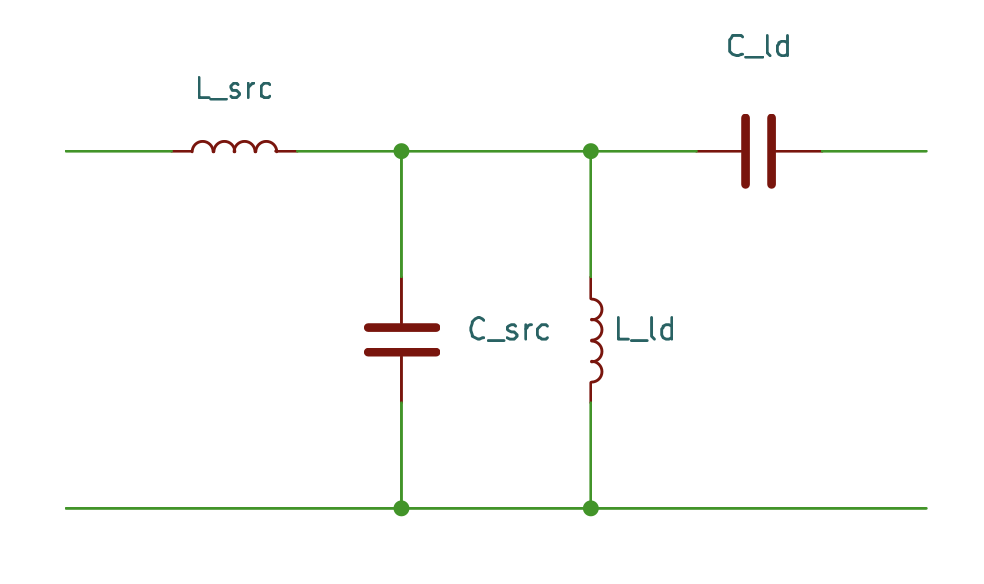
\includegraphics[width = \linewidth]{images/matching_network.png}
\end{columns}
  
\end{frame}

\begin{frame}{S-parameters of the Matching Network\footnote{Simulated using \lstinline|.net| parameter in LTSpice}}
\begin{columns}
  \column{0.5\textwidth}
  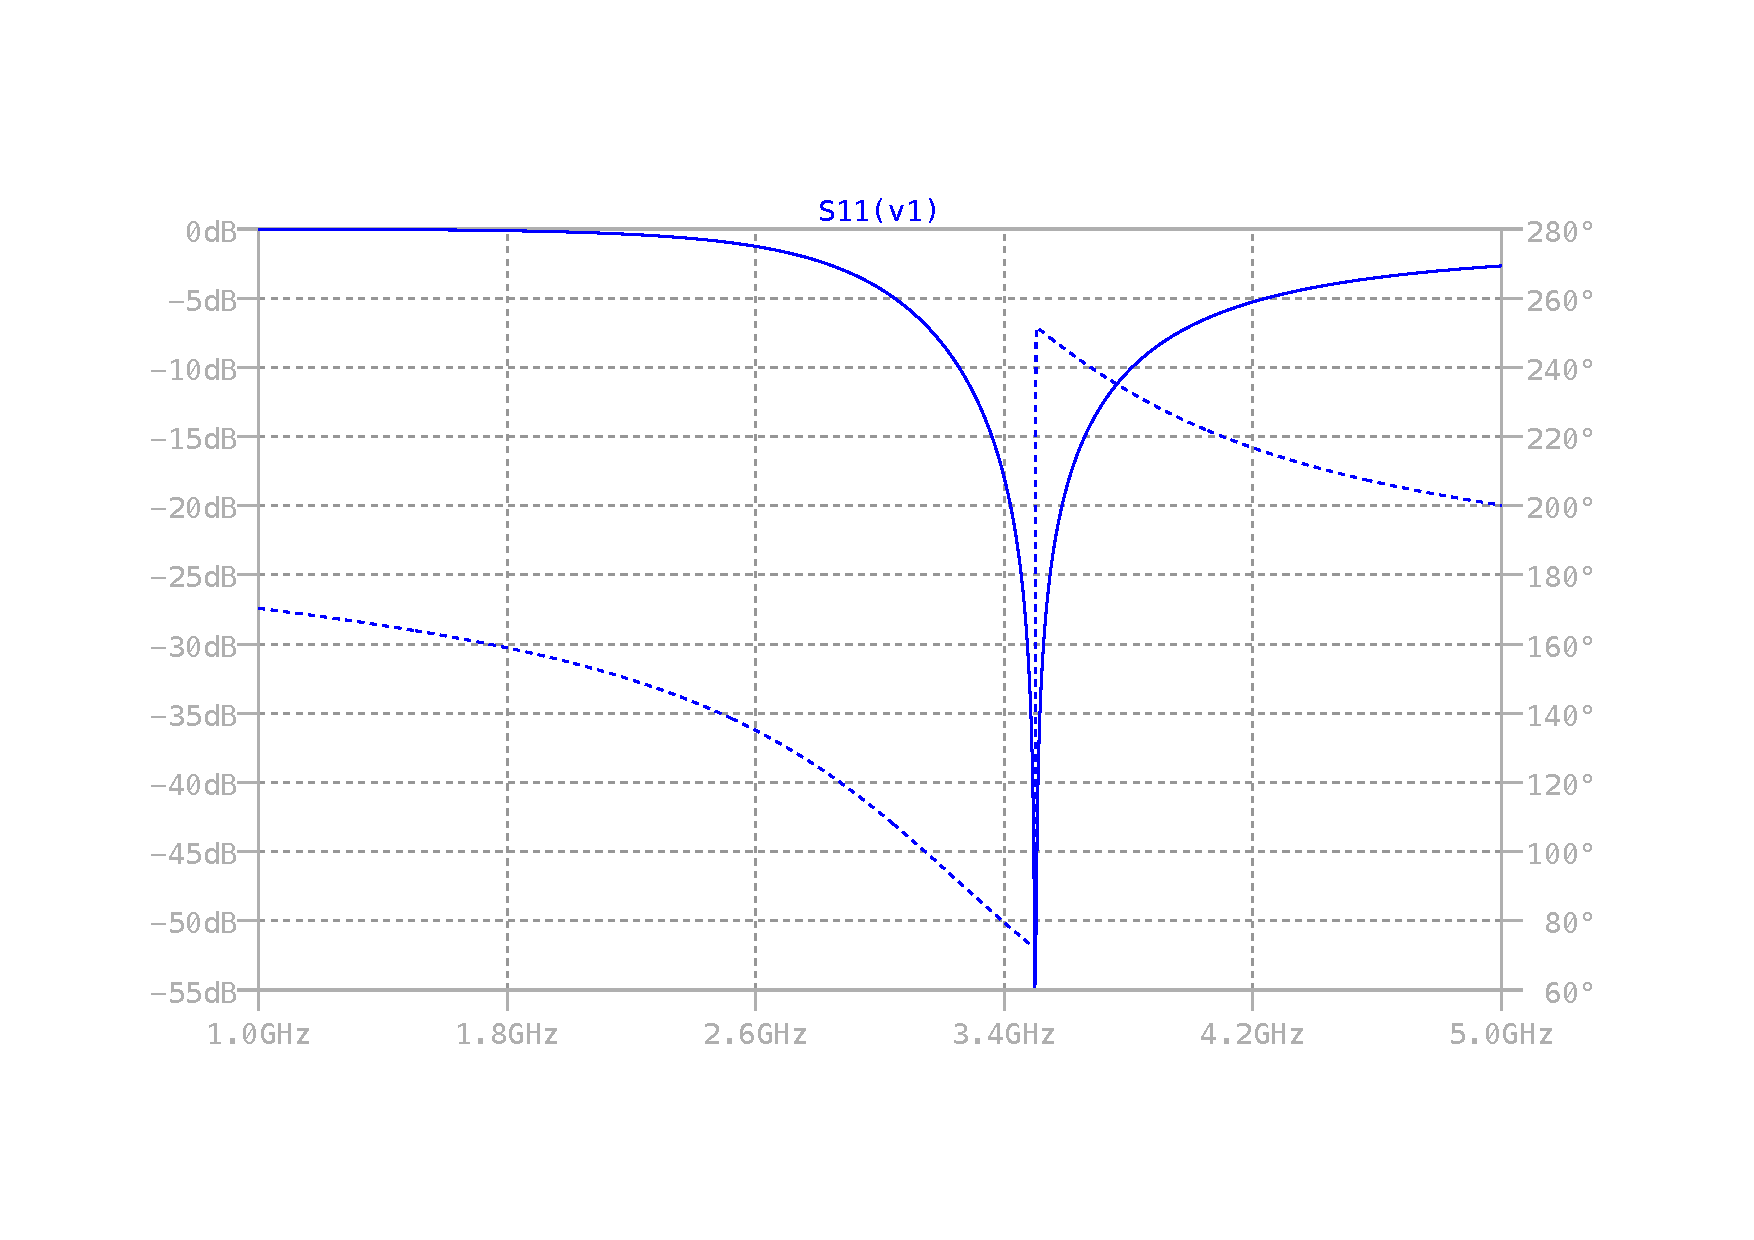
\includegraphics[width=\linewidth]{images/matching_s_params/S11.pdf}
  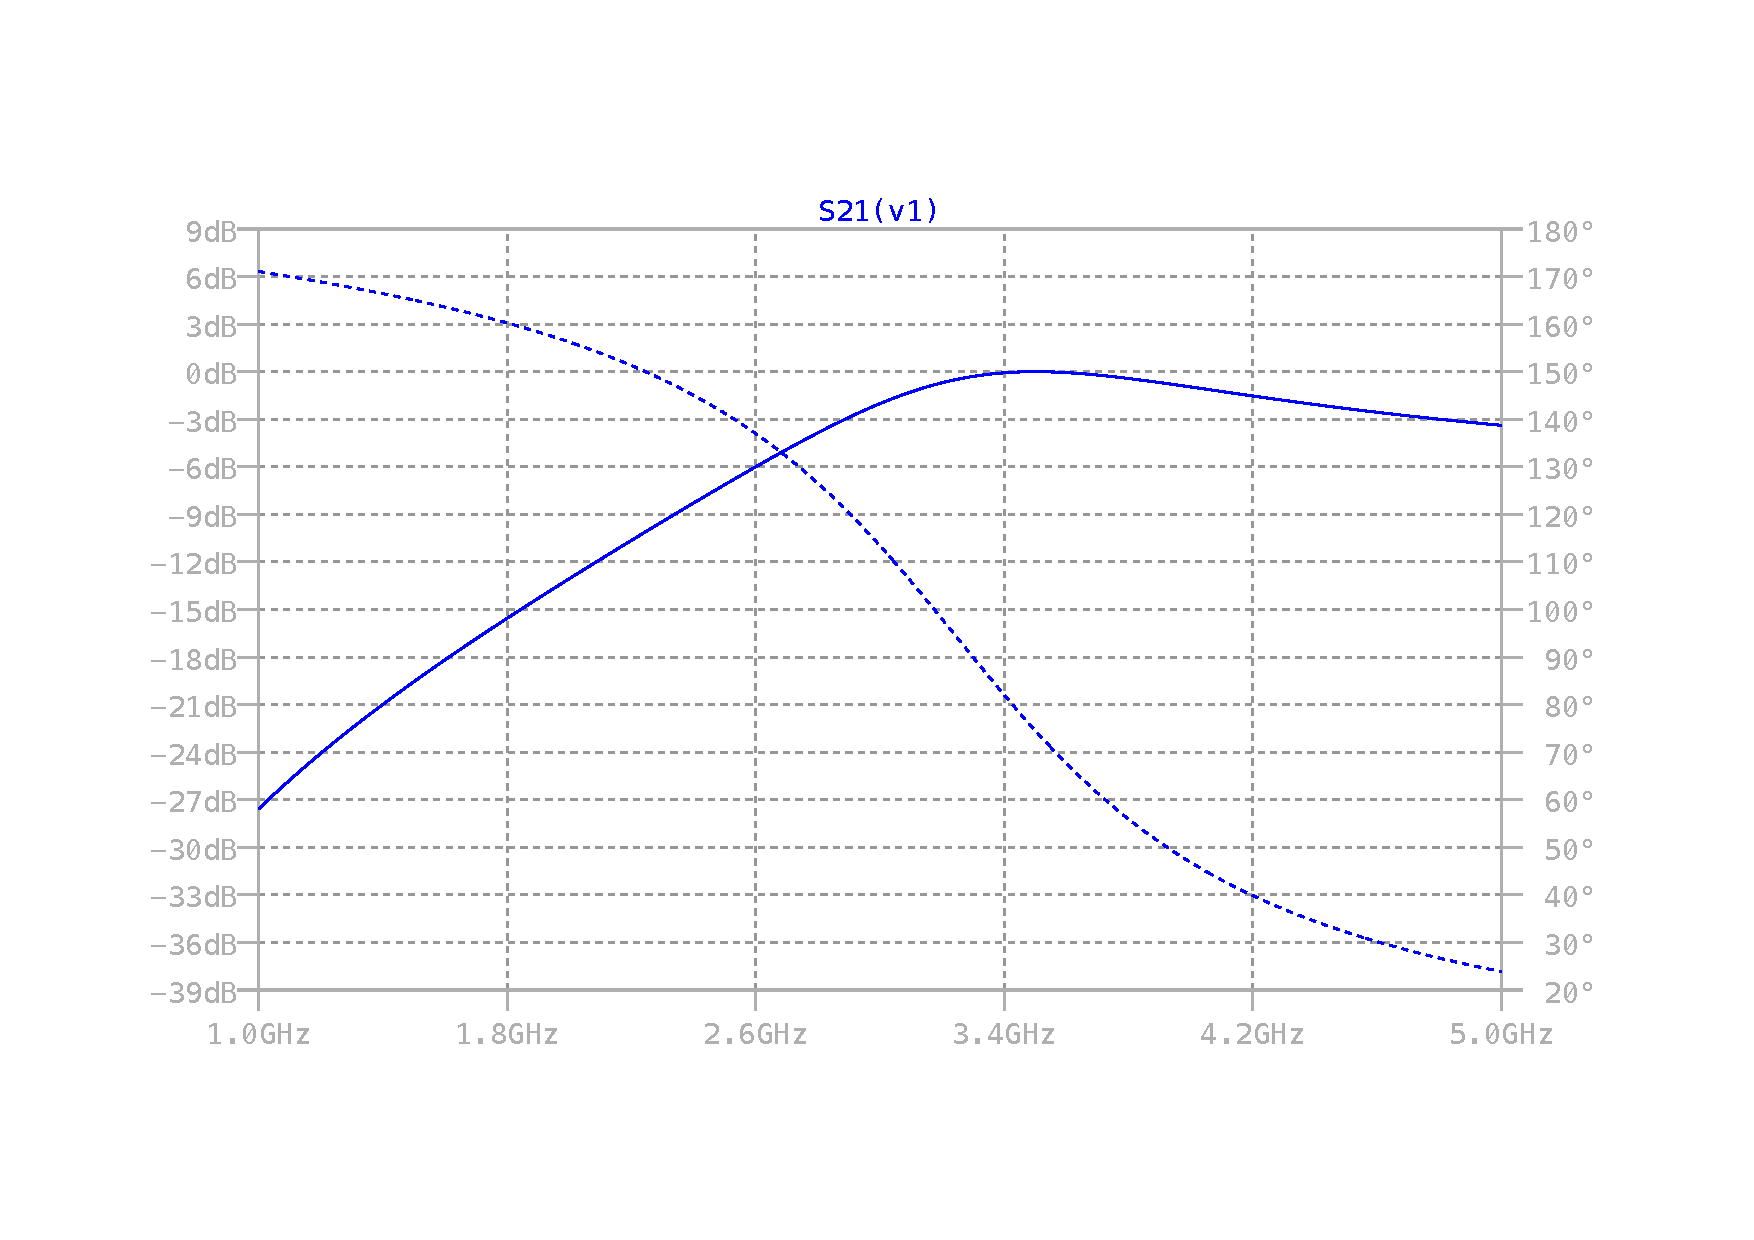
\includegraphics[width=\linewidth]{images/matching_s_params/S21.pdf}
  \column{0.5\textwidth}
  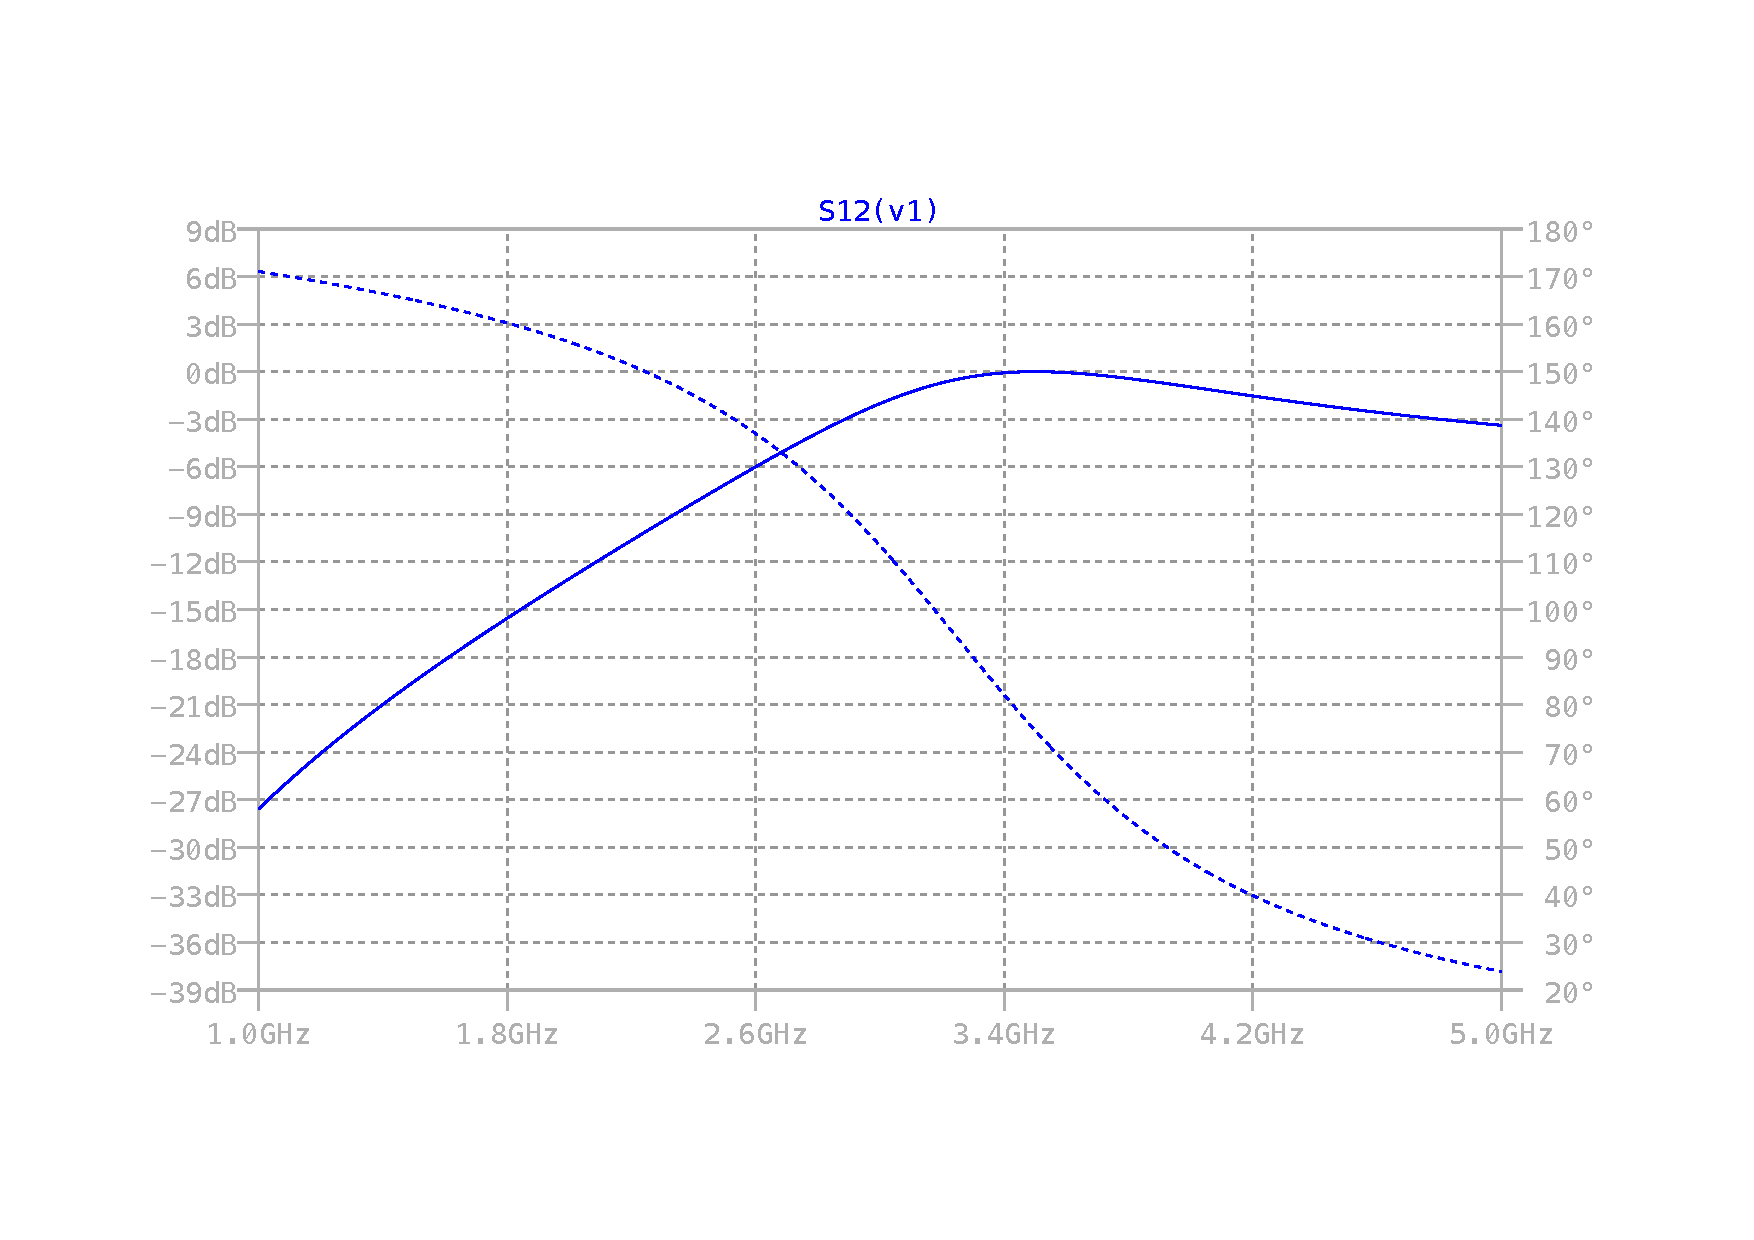
\includegraphics[width=\linewidth]{images/matching_s_params/S12.pdf}
  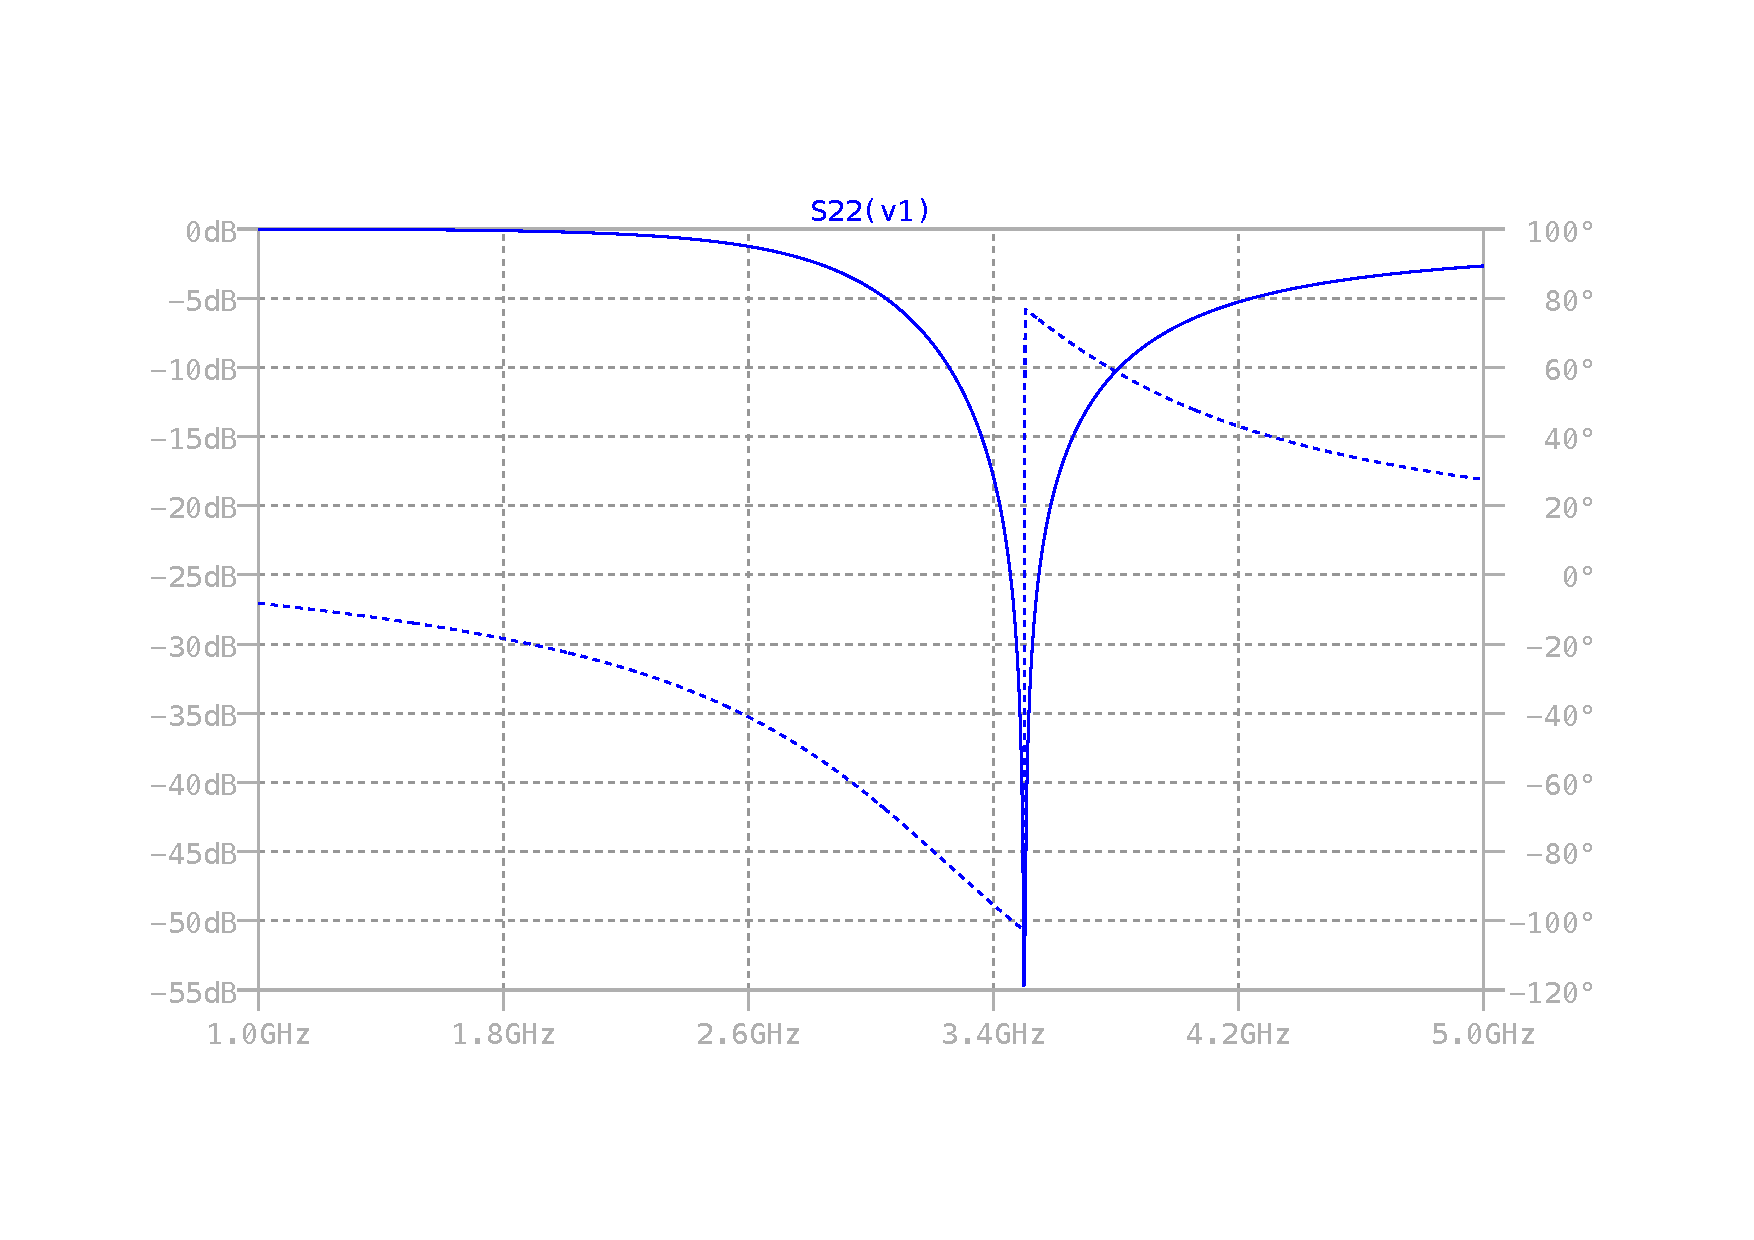
\includegraphics[width=\linewidth]{images/matching_s_params/S22.pdf}
\end{columns}
\end{frame}

\begin{frame}{Input impedance through the Matching Network}
  \begin{itemize}
    \item Attains max value of \(\approx 1000[\Omega]\) at \(3.5[GHz]\)
    \item Tapers quickly for the non-central frequencies
  \end{itemize}
  \begin{center}
    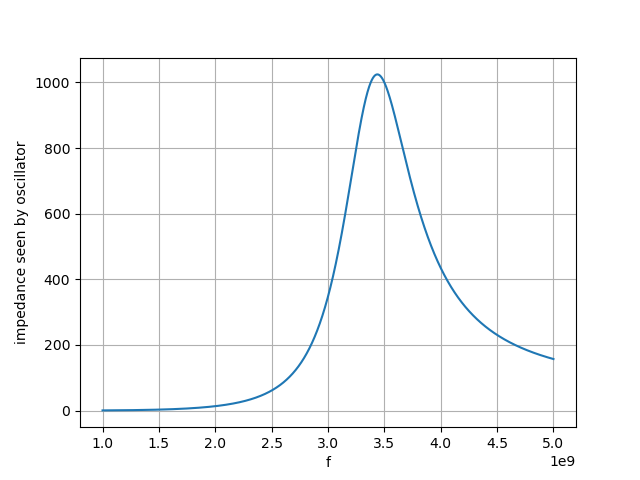
\includegraphics[width=0.6\linewidth]{images/matching_s_params/matching_input_imp.png}
  \end{center}
\end{frame}

\begin{frame}{Oscillator using Matching Network as \(50[\Omega]\) load}
  After making adjustments to supply and current to maximize efficiency, we have the following system\footnote{Efficiency \(\eta\) is defined in the next section}
  \begin{center}
    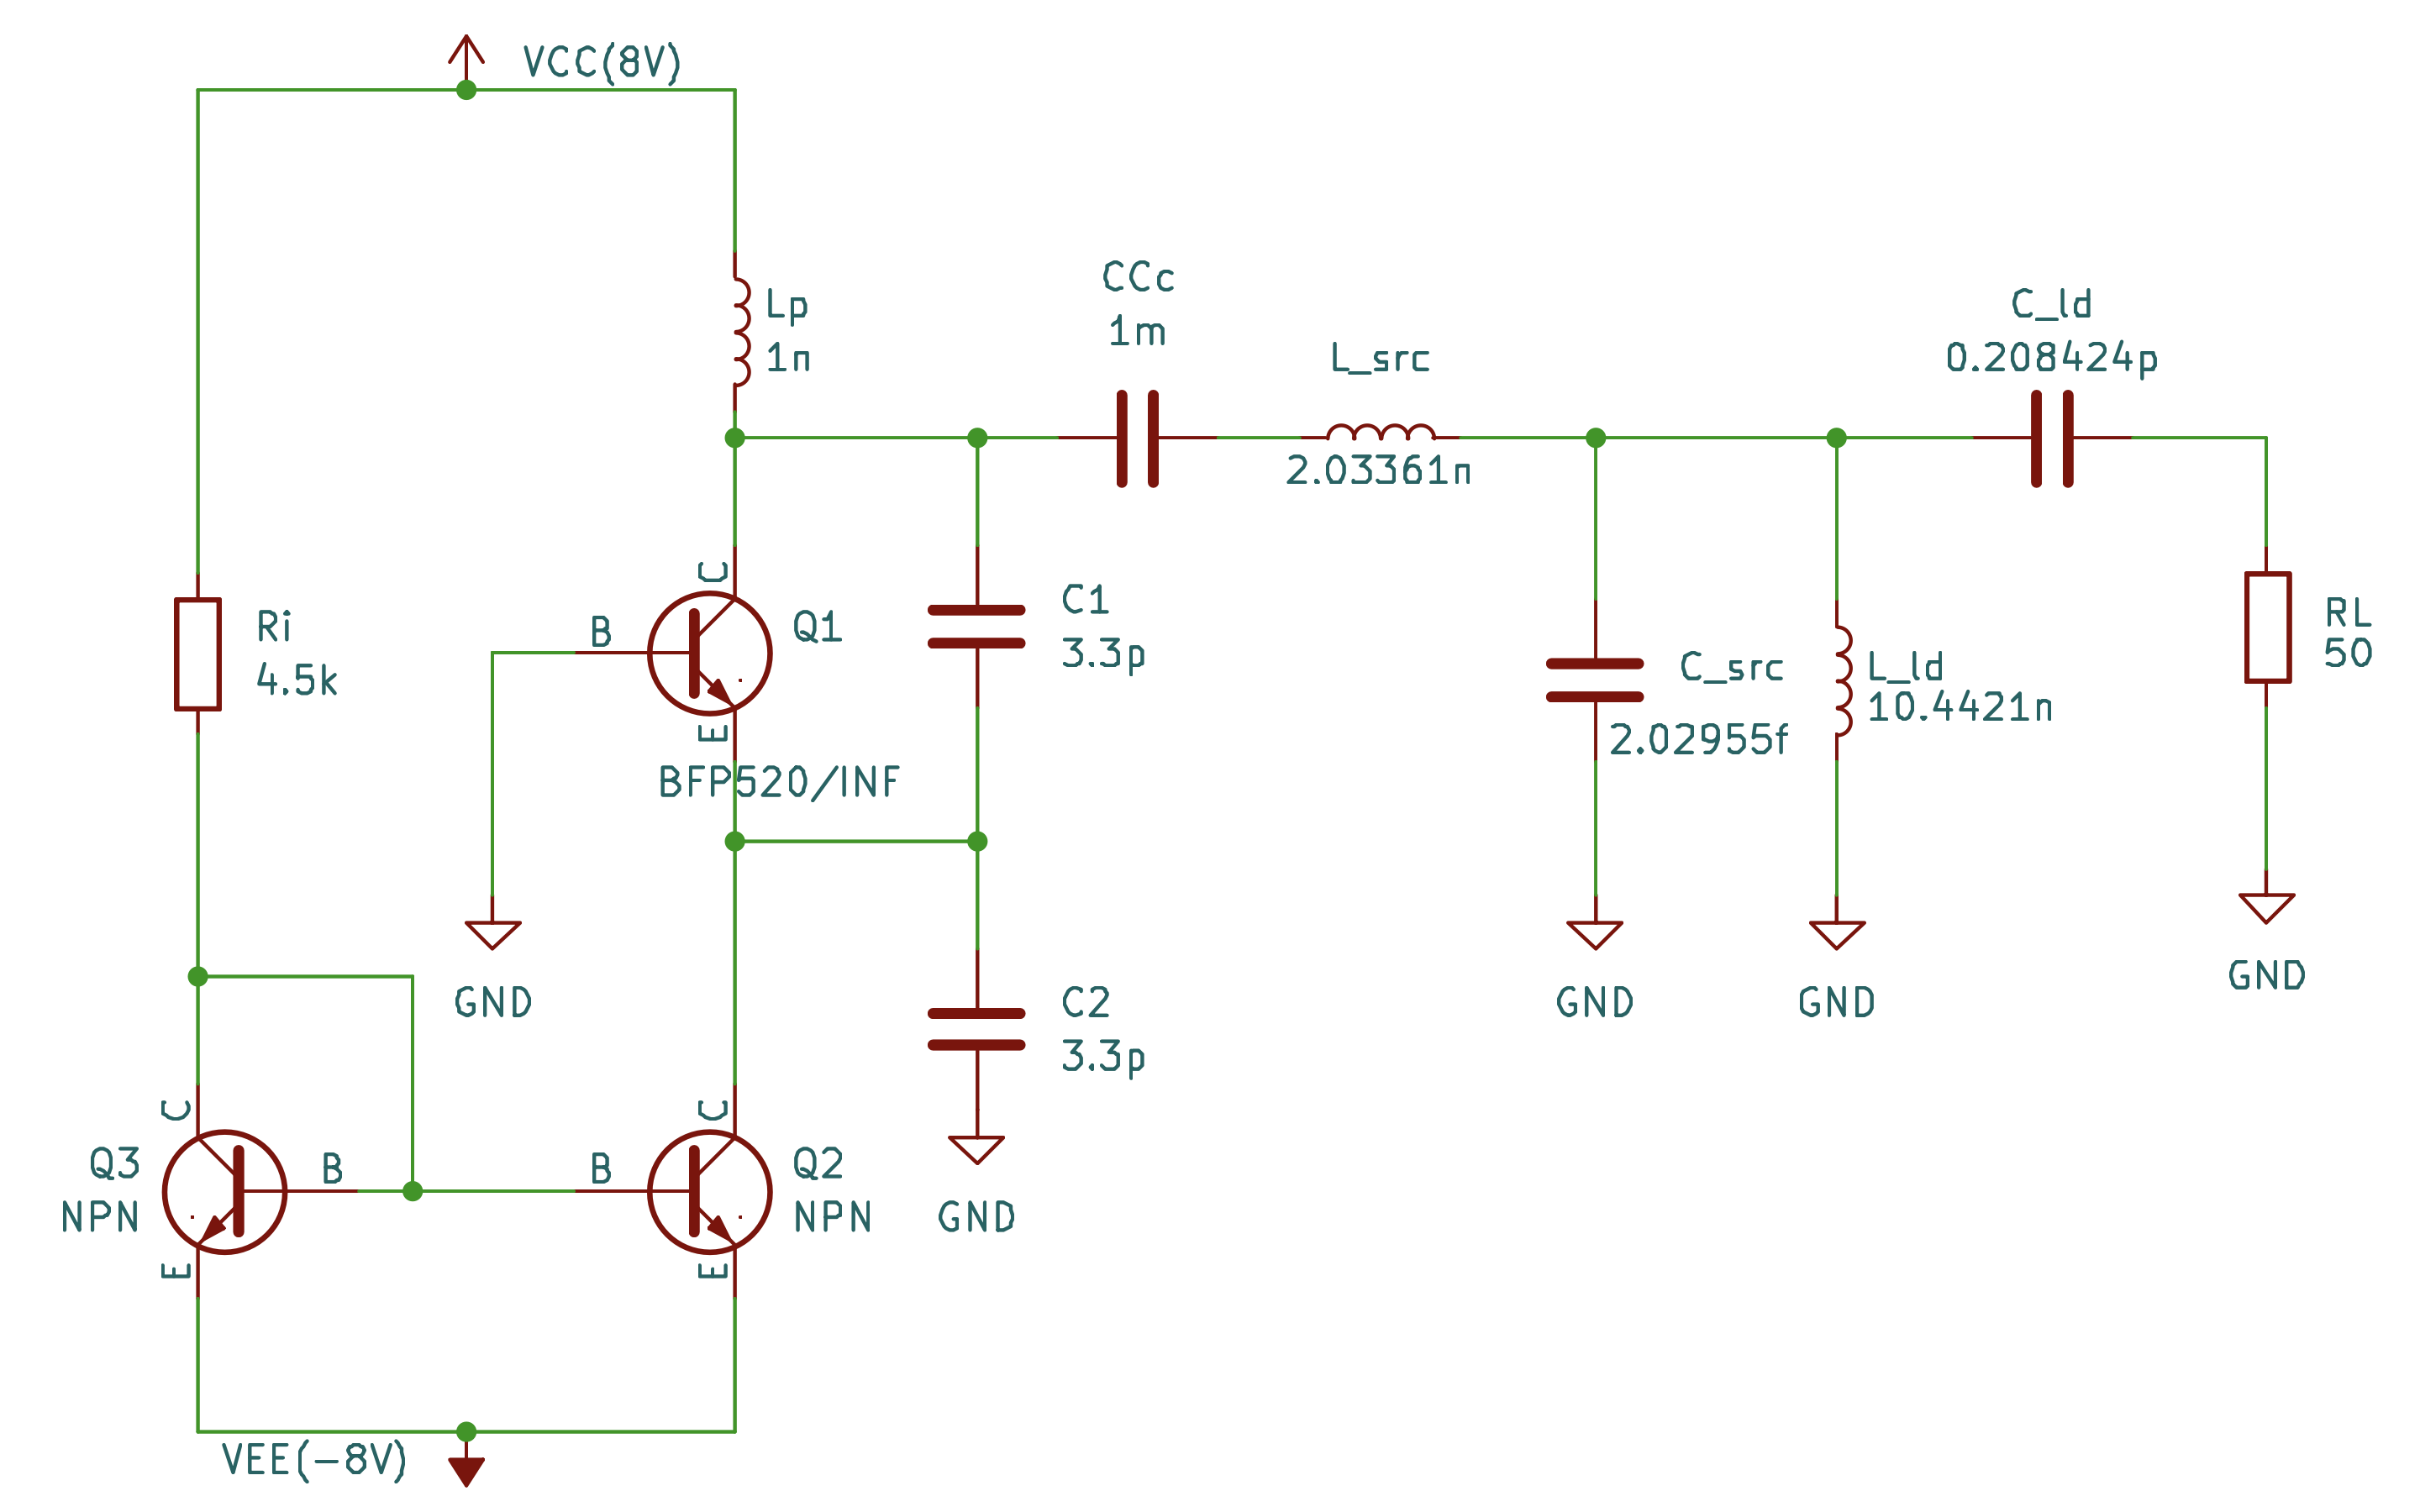
\includegraphics[width=0.85\linewidth]{images/Full_system.png}
  \end{center}
\end{frame}


\begin{frame}{Output of Oscillator using Matching Network as \(50[\Omega]\) load}


\end{frame}

% ----------------- section 5 --------------------

\section{Efficiency}

\begin{frame}{Calculation of \(\eta\)}
\begin{itemize}
  \item <1-> \textbf{Input:} \(P_{DC} = V_{CC}I_C\)
  \item <2-> \textbf{Output:} \(P_{ac} = \frac{V_{rms}^2}{R_L}\) where \(V_{rms}=\frac{V_{max}}{\sqrt{2}}\) for the output waveform
  \item <3-> \textbf{Efficiency:} \(\eta=\frac{P_{ac}}{P_{CD}}\)
\end{itemize}

\visible<4->{For \(V_{cc} = -V_{ee} = 8[V]\), and current mirror set to give \(3.36[mA]\), we have \(v_p = 1.6[V]\), giving us
\begin{equation*}
  \eta \approx 20\%\footnote{It has been shown (Krauss, et al., 1980) that the maximum theoretical efficiency for this oscillator configuration is \(25\%\), implying we have a decent efficiency}
\end{equation*}}
\end{frame}

% ----------------- section 6 --------------------

\section{Antenna Design}
\begin{frame}{Patch Microstrip Antenna}
  \begin{itemize}
    \item <1-> Directional Antenna with good efficiency and high gain when used in an antenna array
    \item <2-> Input impedance of \(50[\Omega]\)
  \end{itemize}
\end{frame}


% ----------------- section 7 --------------------

\section{Next Steps}

\begin{frame}{Next Steps}
\begin{itemize}
  \item <1-> Layout the PCB
  \item <2-> Fabrication and Testing
\end{itemize}
\end{frame}

\section*{Appendix}

\begin{frame}{Data from Infenion - 1}
  \begin{columns}
    \column{0.48\textwidth}
    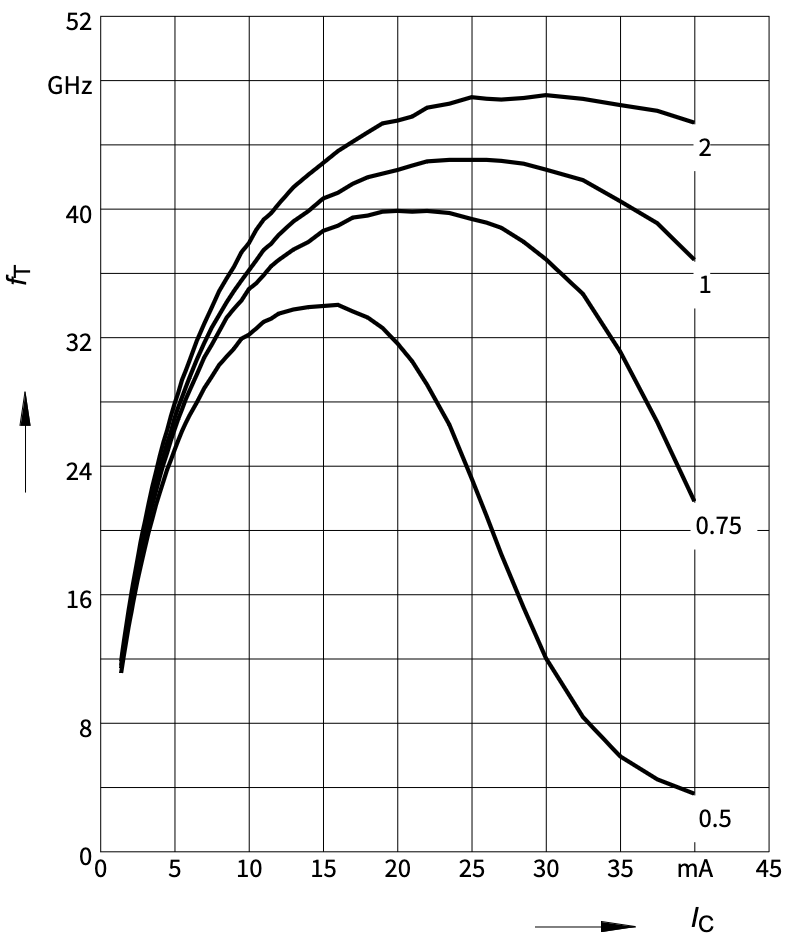
\includegraphics[width=\linewidth]{images/transition_freq_vs_f.png}
    \column{0.48\textwidth}
    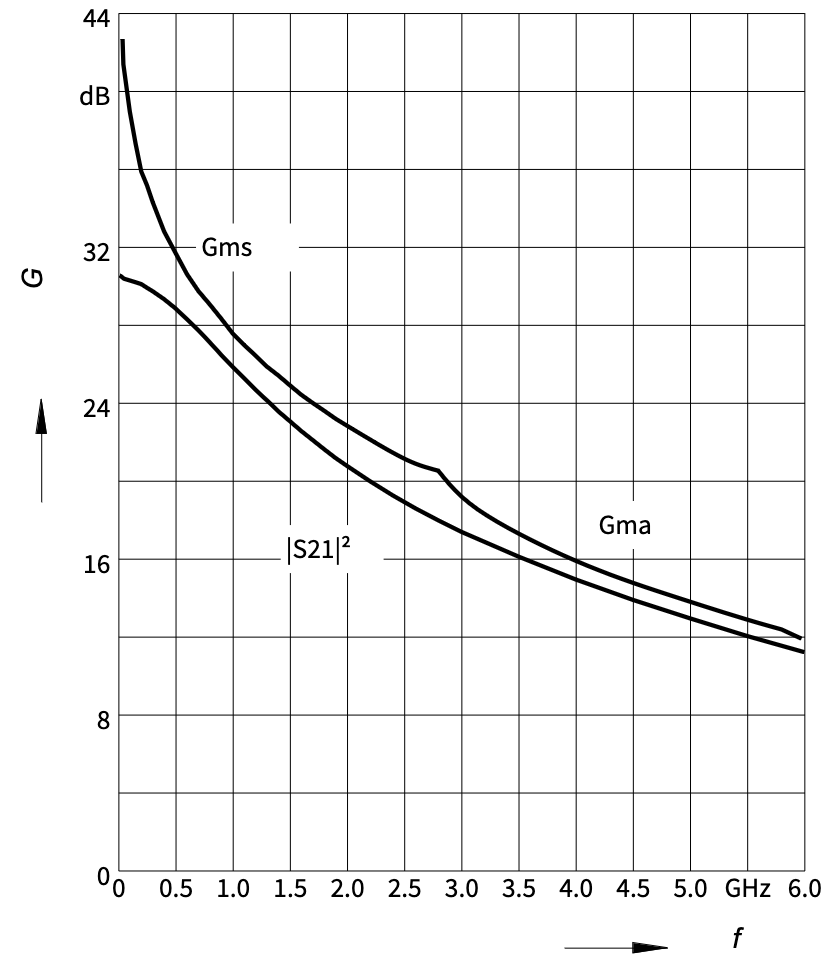
\includegraphics[width=\linewidth]{images/gain_vs_f.png}
  \end{columns}
  \end{frame}
  
  \begin{frame}{Data from Infenion - 2}
  \begin{columns}
    \column{0.48\textwidth}
    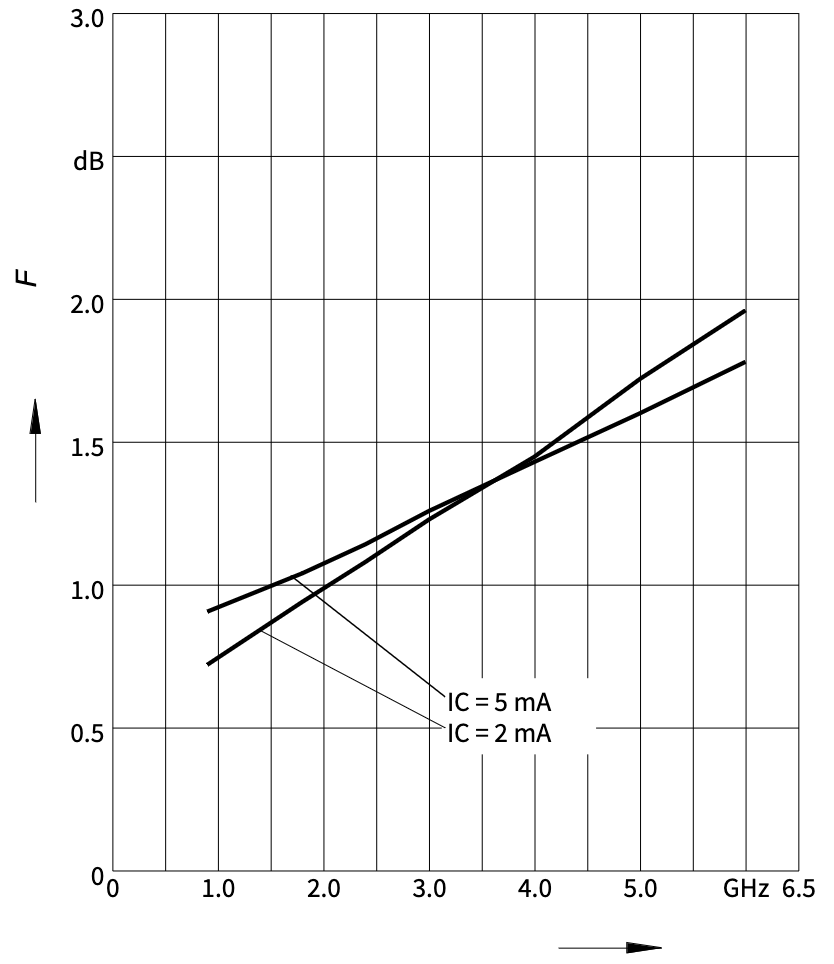
\includegraphics[width=\linewidth]{images/noise_fig_vs_f.png}
    \column{0.48\textwidth}
    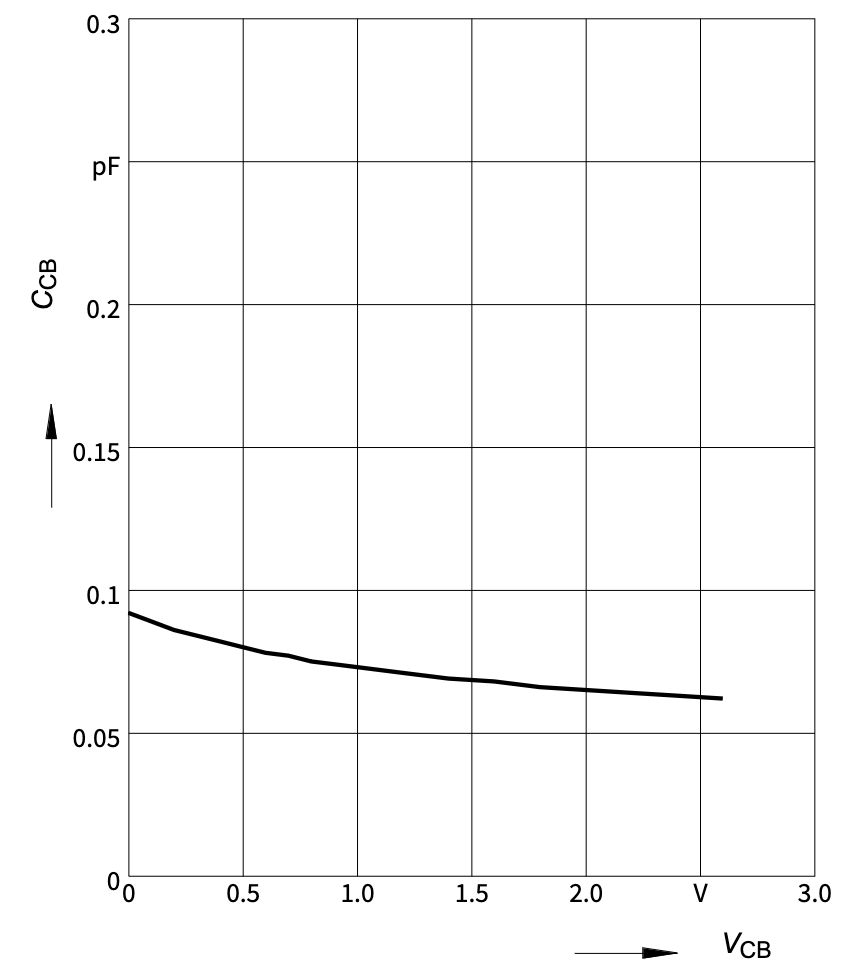
\includegraphics[width=\linewidth]{images/c_cb_vs_f.png}
  \end{columns}
    
  \end{frame}

\begin{frame}[fragile]{BFP520 Spice File}
  \begin{tiny}
    \begin{lstlisting}
      .SUBCKT BFP520/INF 200 100 300
      L1    1   10    0.47nH
      L2    2   20    0.56nH
      L3    3   30    0.23nH
      C1   10   20    6.9fF
      C2   20   30    134fF
      C3   30   10    136fF
      L4   10  100    0.53nH
      L5   20  200    0.58nH
      L6   30  300    0.05nH
      Q1   2 1 3 BFP520
      .ENDS
      .MODEL BFP520 NPN(
      + IS =1.5E-17      NF =1            NR =1
      + ISE=2.5E-14      NE =2            ISC=2E-14
      + NC =2            BF =235          BR =1.5
      + VAF=25           VAR=2            IKF=0.4
      + IKR=0.01         RB =11           RBM=7.5
      + RE =0.6          RC =7.6          CJE=2.35E-13
      + VJE=0.958        MJE=0.335        CJC=9.3E-14
      + VJC=0.661        MJC=0.236        CJS=0
      + VJS=0.75         MJS=0.333        FC=0.5
      + XCJC=1           TF=1.7E-12       TR=5E-08
      + XTF=10           ITF=0.7          VTF=5
      + PTF=50           XTB=-0.25        XTI=0.035
      + EG=1.11)
    \end{lstlisting}
  \end{tiny}
  
  \end{frame}




\begin{frame}{Proof of operating frequency - 1}

  We have the following small signal model of Collpit's oscillator, with \(C_1 = C_2 = C\)\footnote{In all the results, we try to ignore effects of \(r_\pi\) and then adjust the values accordingly to get required response}
  \begin{center}
    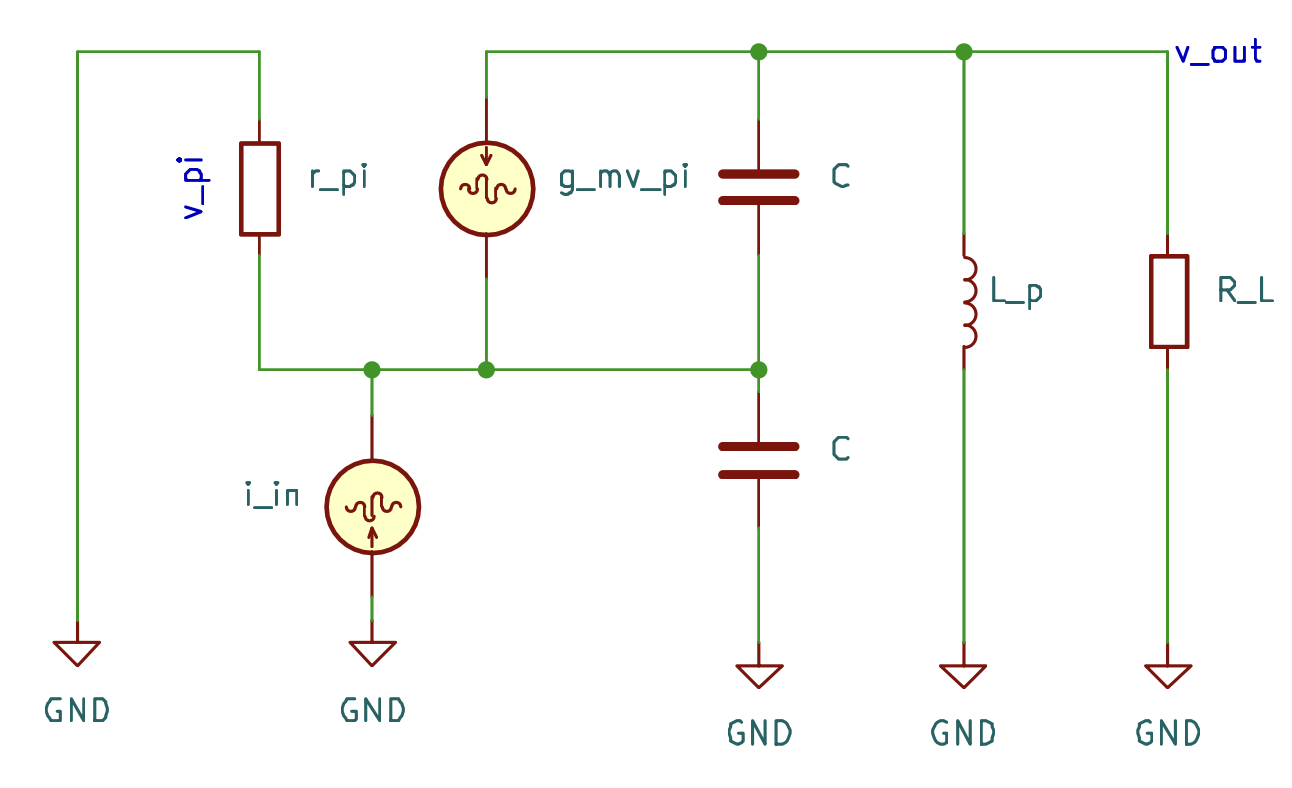
\includegraphics[width = 0.7\linewidth]{images/ssm.png}
  \end{center}
  
\end{frame}

\begin{frame}{Proof of operating frequency - 2}

\begin{equation*}
  i_{in} = -\frac{v_\pi}{r_\pi} - sC(v_{out}+2v_\pi)
\end{equation*}
\begin{equation*}
  g_m v_\pi + sC(v_{out}+v_\pi) + \frac{v_{out}}{sL_p} + \frac{v_{out}}{R_L} = 0
\end{equation*}
This gives us the following frequency response
\begin{tiny}
  \begin{equation*}
    \frac{v_{out}}{i_{in}} = \frac{r_\pi L_p R_L(s^2C + sg_m)}{r_\pi C^2L_p R_L s^3  +(- r\pi C L_p R_L g_m + 2r_\pi CL_p + CL_pR_L)s^2 + (2r_\pi CR_L + L_p)s + R_L}
  \end{equation*}
\end{tiny}

Put \(s = j\omega\) and let \(Im\) of denominator \(\to0\)
\begin{equation*}
  \omega_0 = \sqrt{\frac{2r_\pi CR_L + L_p}{r_\pi C^2 L_p R_L}}
\end{equation*}
Assuming \(r_\pi \to\infty\), as is the case is MOS, we reach the well-known expression \(\omega_0 = \sqrt{\frac{1}{L\frac{C.C}{C+C}}}\)
\end{frame}

\begin{frame}{Proof of operating frequency - 3}

For sustained oscillations, we need
\begin{equation*}
  -(-r_\pi C L_p R_L g_m + 2r_\pi C L_p + CL_p R_L)\omega^2_0 + R_L > 0
\end{equation*}

This gives us
\begin{equation*}\footnote{This is similar to the condition found in Razavi, but for NMOS in place of NPN BJT}
  R_L g_m -\frac{R_L}{r_\pi} -2 > 0
\end{equation*}

Thus, we need to set \(R_L\) accordingly at the oscillating frequency, giving us a lower bound for load and thus a need for a matching network
\end{frame}

\begin{frame}{Calculation of matching network - 1}
\small
We have a source impedance \(Z_s\), a load impedance \(Z_L\), and operating frequency \(f_0\) and we need to match \(Z_L\) to \(Z_s\) at \(f_0\) using a T-Matching Network. We assume a central impedance \(Z_c\) such that \(Z_c > \max(Z_s, Z_L)\), and then calculate the series and parallel reactive components on both sides.\footnote{In our case, all impedances are real}
\begin{columns}
  \column{0.5\textwidth}
  Source:
  \[Q_{src} = \sqrt{\frac{Z_c}{Z_s}-1}\]
  \[X_{src}^{patallel} = \frac{Z_c}{Q_{src}}\]
  \[X_{src}^{series} = Q_{src}Z_s\]
  \column{0.5\textwidth}
  Load:
  \[Q_{ld} = \sqrt{\frac{Z_c}{Z_L}-1}\]
  \[X_{ld}^{patallel} = \frac{Z_c}{Q_{ld}}\]
  \[X_{ls}^{series} = Q_{ls}Z_L\]
\end{columns}
Then, \(L=\frac{X}{2\pi f_0}\) and \(C = \frac{1}{2\pi f_0 X}\) for chosen \(X\) series/parallel
\end{frame}

\begin{frame}[fragile]{Calculation of matching network - 2\footnote{Values generated using \lstinline|.py| script that we made}}
After this, the values of \(V_{cc}, V_{ee}, \) and \(I_c\) were changed so as to get the maximum efficiency. \(R_L\) was matched to \(1[K\Omega]\).
\begin{columns}
  \column{0.45\textwidth}
  \begin{table}
    \centering
    \begin{tabular}{|c|c|}
        \hline
        \textbf{Variable} & \textbf{Value} \\
        \hline
        $f_0$ & $3.5 \times 10^9$ \\
        $Z_{\text{out\_osc}}$ & $1000$ \\
        $Z_{\text{load}}$ & $50$ \\
        $Z_{\text{center}}$ & $1002$ \\
        $Q_{\text{src}}$ & $0.0447214$ \\
        $X_{\text{paralle\_src}}$ & $22405.4$ \\
        $X_{\text{series\_src}}$ & $44.7214$ \\
        $L_{\text{src}}$ & $2.03361 \times 10^{-9}$ \\
        \hline
    \end{tabular}
  \end{table} 
  \column{0.45\textwidth}
  \begin{table}
    \centering
    \begin{tabular}{|c|c|}
        \hline
        \textbf{Variable} & \textbf{Value} \\
        \hline
        $C_{\text{src}}$ & $2.02955 \times 10^{-15}$ \\
        $Q_{\text{ld}}$ & $4.36348$ \\
        $X_{\text{paralle\_ld}}$ & $229.633$ \\
        $X_{\text{series\_ld}}$ & $218.174$ \\
        $L_{\text{ld}}$ & $1.04421 \times 10^{-8}$ \\
        $C_{\text{ld}}$ & $2.08424 \times 10^{-13}$ \\
        $C_{\text{com}}$ & $2.10454 \times 10^{-13}$ \\
        $L_{\text{com}}$ & $1.70212 \times 10^{-9}$ \\
        \hline
    \end{tabular}
  \end{table} 
\end{columns}

\end{frame}

\begin{comment}
  pdflatex yourfile.tex
  bibtex yourfile.aux
  pdflatex yourfile.tex
  pdflatex yourfile.tex
\end{comment}

\begin{frame}{Calculation of parameters of Patch Antenna}
  \begin{columns}
    \column{0.5\textwidth}
      \begin{enumerate}
        \item <1->\(W = \frac{1}{2f\sqrt{\mu_0\epsilon_0}}\sqrt{\frac{2}{\epsilon_r+1}}\)
        \item <2-> \(\epsilon_{eff} = \frac{\epsilon_r+1}{2} + \frac{\epsilon_r - 1}{2\sqrt{1+\frac{12h}{W}}}\)
        \item <3-> \(\frac{\Delta L}{h} = 0.412\frac{(\epsilon_{eff} + 0.3)\left(\frac{W}{h} + 0.264\right)}{(\epsilon_{eff} - 0.258)\left(\frac{W}{h} + 0.8\right)}\)
      \end{enumerate}
    \column{0.5\textwidth}
  \end{columns}
\end{frame}

\begin{frame}[allowframebreaks]{References}
  \nocite{*}
  \bibliographystyle{ieeetr}
  \bibliography{references.bib}
\end{frame} 

\end{document}